\documentclass[hidelinks, 12pt]{report}
\usepackage{graphicx}
\usepackage{marginnote}
\usepackage{amsmath}
\usepackage{amssymb}
\usepackage{geometry}
\usepackage[document]{ragged2e}
\usepackage[utf8]{inputenc}
\usepackage[english]{babel}
\usepackage{fancyhdr}
\usepackage{float}
%\usepackage{floatrow}
\usepackage{caption}
%\usepackage{calc}
\usepackage{chngcntr}
\usepackage[caption = false]{subfig}
\usepackage[subfigure]{tocloft}
\newlength{\mylen}
\usepackage[font=footnotesize,labelfont=bf]{caption}
%\usepackage{times}
\usepackage[table]{xcolor}
\usepackage[intoc]{nomencl}
\usepackage{setspace}
\usepackage{tocloft}

%\usepackage{nomencl}
%\let\abbrev\nomenclature
%\makenomenclature 
%\newcommand{\Abkuerzung}{
%\printnomenclature
%\newpage
%}


\usepackage{array}
\usepackage{hyperref}
\hypersetup{
    colorlinks=true,
    linkcolor=blue,
    filecolor=green,      
    urlcolor=cyan,
    citecolor=magenta,
}
\urlstyle{same}
\usepackage{bookmark}
\renewcommand{\cftfigpresnum}{\figurename\enspace}
\renewcommand{\cftfigaftersnum}{:}
\settowidth{\mylen}{\cftfigaftersnum\cftfigpresnum}
\addtolength{\cftfignumwidth}{\mylen}
\counterwithin{figure}{section}

\renewcommand{\cfttabpresnum}{\tablename\enspace}
\renewcommand{\cfttabaftersnum}{:}
\settowidth{\mylen}{\cfttabaftersnum\cftfigpresnum}
\addtolength{\cfttabnumwidth}{\mylen}
\counterwithin{table}{section}

\renewcommand{\labelenumi}{(\roman{enumi})}

\geometry{margin=1in}

\usepackage{titlesec}
\titleformat{\chapter}[display]
{\normalfont %
    \Huge % %change this size to your needs for the first line
    \bfseries}{\chaptertitlename\ \thechapter}{20pt}{%
    \huge} %change this size to your needs for the second line
 


\fancyhf{}
\fancyhead[LE,LO]{\footnotesize{}}
\fancyhead[RE,RO]{\footnotesize{Communications and Signals Design for Wireless Power Transmission}}
\fancyfoot[LE,LO]{\footnotesize{Govt. Model Engineering College}}
\fancyfoot[RE,RO]{\footnotesize\thepage}
\renewcommand{\headrulewidth}{1pt}
\renewcommand{\footrulewidth}{1pt}
%\renewcommand{\familydefault}{\rmdefault}
\newcommand{\Rnum}[1]{\uppercase\expandafter{\romannumeral#1}}
\newcommand{\rnum}[1]{\romannumeral#1\relax}
%\setcounter{secnumdepth}{4}
%\setcounter{tocdepth}{4}

\begin{document}
\pagenumbering{none}
\centering
\section*{\centering{Bonafide Certificate}}
\vspace{1cm}

\includegraphics[height=3cm,width=3cm]{logo}

\begin{center}
MODEL ENGINEERING COLLEGE\\
\vspace{0.5cm}
THRIKKAKARA, KOCHI-21\\
\vspace{0.5cm}
DEPARTMENT OF ELECTRONICS AND COMMUNICATION \\
\vspace{0.5cm}
APJ ABDUL KALAM TECHNOLOGICAL UNIVERSITY \\
\vspace{1cm}
\textit{Bonafide Certificate}
\\This is to Certify that the Seminar Report entitled\\
\vspace{0.5cm}
\textbf{Communications and Signals Design for Wireless Power Transmission} 
\\
\vspace{0.5cm}
Submitted by\\
\vspace{0.2cm}
M.G. Krishnan\\
\vspace{0.2cm}
is a bonafide account of his work done under our supervision. \\
\end{center}

\vspace{2cm}
\begin{minipage}[t]{10cm}
\flushleft \textbf{Seminar Co-ordinator}\\
Prof. Sunith C.K.\\
Assistant Professor\\
Dept. of Electronics and\\
Communication Engineering
\end{minipage}
\vspace{2cm}
\begin{minipage}[t]{5cm}
\flushleft \textbf{Seminar Guide}\\
Prof. Arun C.R.\\
Assistant Professor\\
Dept. of Electronics and\\
Communication Engineering
\end{minipage}
%\begin{minipage}[t]{5cm}
%\flushleft Head of Department\\
%Mr. Pradeep M\\
%Associate Professor\\
%\end{minipage}

%\addcontentsline{toc}{chapter}{Abstract}
\chapter*{Abstract}
\justify
\textit{
Radiative wireless power transfer (WPT) is a promising technology to provide cost-effective and real-time power supplies to wireless devices. Although radiative WPT shares many similar characteristics with the extensively studied wireless information transfer or communication, they also differ significantly in terms of design objectives, transmitter/receiver architectures and hardware constraints, etc. An overview on the various WPT technologies, the historical development of the radiative WPT technology and the main challenges in designing contemporary radiative WPT systems is given. The state-of-the-art communication and signal processing techniques that can be applied to tackle these challenges are also discussed. Topics discussed include energy harvester modeling, energy beamforming for WPT, channel acquisition, power region characterization in multi-user WPT, waveform design with linear and non-linear energy receiver model, safety and health issues of WPT, massive MIMO (multiple-input multiple-output) and millimeter wave (mmWave) enabled WPT, wireless charging control, and wireless power and communication systems codesign. Directions that are promising for future research are also discussed.}\\

\textit{\textbf{keyword}}- 
Wireless power transfer, energy beamforming, channel estimation and feedback, non-linear energy harvesting model, waveform design.
%\end{keyword}
%\sep%

\pagebreak
\setcounter{page}{1}
\pagenumbering{roman}
\justify
%\onehalfspacing
\begin{spacing}{0.8}
\renewcommand{\contentsname}{Table of Contents}
\pdfbookmark{\contentsname}{Table of Contents}
\tableofcontents
\end{spacing}
\pagebreak
%line spacing
\addcontentsline{toc}{chapter}{List of Figures}
\listoffigures 
\pagebreak
\renewcommand{\nomname}{List of Abbreviations}
\addcontentsline{toc}{chapter}{List of Abbreviations}
\printnomenclature
\pagebreak
%\addcontentsline{toc}{chapter}{List of Tables}
%\listoftables
%\pagebreak

\section*{List of Abbreviations}
\begin{flushleft}
WPT -  Wireless Power Transfer\\ 
\vspace{0.5cm}
MIMO - Multiple Input Multiple Output\\
\vspace{0.5cm}
LoS - Line of Sight\\
\vspace{0.5cm}
SWIPT - Simultaneous Wireless Information and Power Transfer\\
\vspace{0.5cm}
ET - Energy Transmitter\\
\vspace{0.5cm}
ER - Energy Receiver\\
\vspace{0.5cm}
RF - Radio Frequency\\
\vspace{0.5cm}
CSI - Channel State Information\\
\vspace{0.5cm}
SPS - Solar Power Satellite\\
\vspace{0.5cm}
OFDM - Orthogonal Frequency Division Multiplexing\\
\end{flushleft}
\pagebreak

\addcontentsline{toc}{chapter}{Acknowledgement}
\section*{Acknowledgement}
\justify
On the recollection of so many great favors and blessings, I offer my sincere thanks to the Almighty, the Creator and Preserver.\\
%\vspace{1cm}

I express my heartfelt gratitude to \textbf{Prof. Dr. V P Devassia}, Principal, Govt. Model Engineering College, Thrikkakara for providing me with excellent library facilities. \\
I am thankful to my seminar coordinator \textbf{Mr. Sunith C. K.}, Assistant Professor, Department of Electronics and Communication Engineering, and \textbf{Mrs. Swapna P. P.}, Assistant Professor, Department of Electronics and Communication Engineering for the full-fledged support and guidance. I sincerely thank \textbf{Prof. Arun C.R.} , Assistant Professor of Department of Electronics and Communication Engineering, for his timely advice and motivating me to do everything in a better way.\\

Last but not the least I am thankful to one and all of the Department of Electronics and Communication Engineering and the whole library staff for their co-operation and active involvement. I also thank my colleagues for their support.
\hbox{} \newpage 
\pagenumbering{arabic} 
\pagestyle{fancy}
\chapter{Introduction}
\justify
All kinds of electronic devices consume some form of energy or the other for its functioning. Devices such as cell phones, cameras, and laptops are powered by batteries, which have limited energy storage capacity. These batteries need to be regularly replaced or recharged. With the increase in use of portable devices such as cell phones, the need for powering up them wirelessly has also increased. Wireless charging can eliminate the need of connecting wires, can prove to be cost effective in the long run, avoids massive battery disposal and can be used in hazardous conditions. The key enabler for wireless charging is the advancement of wireless power transfer (WPT) technology. WPT refers to the technology of delivering power from a source to destination without interconnecting wires. Various WPT technologies have been developed so far, including inductive coupling, magnetic resonant coupling, electromagnetic radiation, and laser power beaming, among others. Right from 1880s, WPT has been in research with Heinrich Hertz demonstrating the existence and propagation of electromagnetic waves in free sapce. Advancements in microwave technology gave WPT the required boost. The development of magnetron tubes for highpower microwave generations and more advanced parabolic antennas for highly directional radiations helped bring advancements to the technology. Significant advancements have been made in the field of Magnetic Resonant Coupling WPT and Inductive Coupling WPT. However, these technologies are limited with short range, lower efficiency at longer range, size of transmitters and receivers. Radiative WPT on the other hand, increased the range significantly, eliminates the need for Line of Sight transmission and enables use of Multiple Input Multiple Output (MIMO). Radiative WPT also allows high power transmissions and can be used in Solar Power Satellite (SPS). 
\begin{figure}[H]
\centering
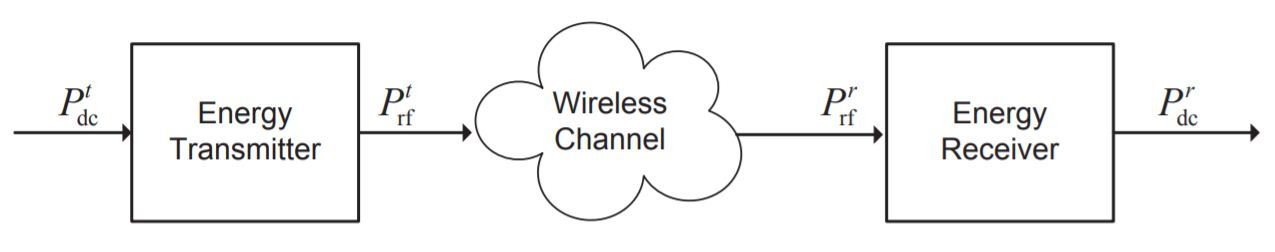
\includegraphics[width=15cm,height=5cm]{Block.JPG}
\caption[Method Overview]{Method Overview}
\label{Method Overview}
\end{figure}
\chapter{Literature Survey}
\section{Existing Methods and Drawbacks}
\justify
Various WPT technologies have been developed so far, including inductive coupling, magnetic resonant coupling, electromagnetic (EM) radiation, and laser power beaming, among others. 
Inductive coupling is a near-field WPT technology where power is transferred between two properly aligned transmitter/receiver coils by magnetic field. The fundamental principles of inductive WPT are Ampere’s law and Faraday’s law of induction. The alternating current passing through the transmitter coil creates a timevarying magnetic field, which, upon passing through the receiving coil, induces an alternating current in the receiving circuit that could be converted to usage energy. Inductive coupling is able to achieve high power transfer efficiency, but the transmitter and receiver need to be in close proximity and aligned accurately. Thus, inductive coupling is not suitable for charging multiple devices concurrently when the devices are freely placed in an area.
Magnetic resonant coupling is another near-field WPT technology that makes use of resonant coupling. Two objects resonant at the same frequency tend to couple with each other most efficiently. Magnetic resonant coupling is able to achieve higher power transfer efficiency over longer distances than inductive coupling. WPT via magnetic resonant coupling has a relatively loose requirement on coil alignment. This technology also requires large sized transmitters and receivers.
Laser power beaming uses highly concentrated laser light aiming at the energy receiver to achieve efficient power delivery over long distances. The receiver of laser powering uses specialized photovoltaic cells to convert the received laser light into electricity. One promising application of laser-based WPT technology is to provide essentially perpetual power supply to unmanned aerial vehicles (UAVs) in flight, enabling them potentially unlimited endurance aloft. However laser radiation could be hazardous. Laser beaming requires LoS link as well as accurate pointing towards the receiver, which could be challenging to achieve in practice. Laser beaming is vulnerable to atmospheric absorption and scattering by clouds, fog, and rain, which greatly hinders its practical applications.
\section{Proposed Method}
\justify
Radiative WPT is a far-field wireless power transmission technology with the transmitter and receiver completely decoupled electrically. In radiative WPT, the modulated/unmodulated energy-bearing signals at the transmitter are up-converted into the designated radio frequency, radiated by the transmitting antennas, propagating through the wireless channel, then picked up by the receiving antennas, and finally converted into the usable direct current via devices such as rectifiers. The combination of the energy receiving antenna and the rectifier is termed rectenna. Depending on the antenna size, transmitting power, as well as the propagation environment, radiative WPT may achieve power delivery over distances varying from a few meters to even hundreds of kilometers. It also allows transmission in non Line of Sight environment and simultaneous wireless information and power transfer. Radiative WPT has a wide range of applications, spanning from low-power wireless charging for devices such as radio frequency identification tags, wireless sensors, Internet of Things devices, and consumer electronics, to high-power applications such as microwavepowered aircrafts as well as SPS. 

The important engineering requirements as well as the main design challenges for future radiative WPT systems.
\begin{itemize}
\item{Range: Future WPT systems are expected to achieve power delivery for distances from a few meters to hundreds of meters.}
\begin{itemize}
\item{Efficiency: The end-to-end power transfer efficiency is of paramount importance. This requires efficient DC to RF power conversion at the transmitter, highly directive RF transmission over the air, and highly efficient RF to DC conversion at the receiver.}
\begin{itemize}
\item{Non-line of sight: The ability to support Non Line of Sight power transmission would significantly widen the practical applications of future WPT systems }
\begin{itemize}
\item{Mobility support: Effective radiative WPT systems need to support power delivery even for moving receivers.}
\begin{itemize}
\item{Inter-operate with wireless communication systems: The possibility of transmitting power and information using the same wireless system can significantly boost Power and Communication fields.}

\chapter{System Models and Analysis}
\justify
The aim is to develop an efficient system for transmission of power and information simultaneously using the same system. Efficient
wireless power and communication systems share several similar characteristics and hence similar techniques can be used. Fig. 1.0.1 shows a generic WPT system, which consists of an energy transmitter (ET) and an energy receiver (ER) that are separated by a wireless medium. At the ET, the DC (or lowfrequency AC) energy-bearing signal is up-converted into the RF signal in a designated frequency band and radiated into the air by using transmitting antenna or antenna array. After propagating via the wireless channel, the RF signal arriving at the ER is picked up by the receiving antenna or antenna array, and then converted into usable DC power by rectifier. Denote by Ptdc and Ptrf the input DC power and output RF power at the ET, and Prrf and Prdc the input RF power and output DCpower at the ER, respectively. The end-to-end power transfer efficiency e can be expressed as <equation>. Maximizing Prdc reduces to maximizing the incident RF power Prrf, or equivalently the RF-to-RF transmission efficiency e2.

\section{Antenna Model}
\justify
The antenna model reflects the power transfer from the antenna to the rectifier through the matching network. As illustrated in Fig. 2, a lossless antenna can be modelled as a voltage source vs(t) followed by a series resistance Rant (right). Let Zin = Rin + jXin denote the input impedance of the rectifier with the matching network. Assuming perfect matching, all the available RF power Prrf is transferred to the rectifier and absorbed by Rin, so that vin(t) = vs(t)/2. 
\section{Rectifier and Diode Model}
\justify
Consider a single receive antenna and a rectifier composed of a single series diode followed by a low-pass filter with load as shown in Fig. 2.  Denoting the voltage drop across the diode as vd(t) = vin(t)−vout(t) where vin(t) is the input voltage to the diode and vout(t) is the output voltage across the load resistor. 
\section{Single User WPT}
\justify
A single-user point-to-point MIMO WPT system in the general multi-path environment is considered with multiple antennas at the transmitter and receiver. We assume that a total of N orthogonal sub-bands are used, where the nth sub-band has carrier frequency fn and equal bandwidth Bs, n = 1, · · · , N. 
<equation>











\chapter{Conclusion}
\justify
Under the linear energy harvesting model, the main techniques for enhancing the RF power transfer efficiency are firstly discussed in single-user WPT systems, including energy beamforming, channel acquisition, retrodirective amplification, etc. For multi-user WPT systems, the various networking architectures with different levels of cooperation among the ETs are then introduced, followed by the power region characterizations via convex optimization techniques. The nonlinear energy harvesting model and the corresponding waveform optimizations to further enhance the power transfer efficiency are presented next. Finally, we provide further discussions on various other topics pertaining to WPT, including safety and health issues, WPT using massive MIMO and mmWave techniques, wireless charging control, and wireless power and communication systems co-design. It is hoped that the techniques presented in this article will help inspiring future researches in this exciting area as well as paving the way for practically designing and implementing efficient WPT systems in the future.


\chapter{Future of Radiative WPT}
\justify
The following details need to be considered during advancement of radiative wireless power transfer in future.

\begin{itemize}
\item{Safety and Health Issues: Like any other RF-based wireless systems, WPT systems need to comply with the various safety guidelines to minimize the potential biological effects caused by RF energy. High level RF exposure is harmful to human body due to the rapid heating and thus possibly causes damage to biological tissue. Two widely adopted measures on RF exposure are specific absorbtion rate (SAR) and maximum permissible exposure (MPE), which could be taken into account for WPT systems design. SAR is a measure of the rate at which energy is absorbed by the human body when exposed to RF field.  MPE is defined as the highest level of RF exposure to which a person may be exposed without incurring an established adverse health effect.}
\begin{itemize}
\item{Massive MIMO and MmWave WPT: Massive MIMO is a key enabling technology for the fifth-generation (5G) wireless communication systems by tremendously increasing the spectrum efficiency via deploying a large number of antennas. , massive MIMO is also an appealing technique to enhance the end-to-end power transfer efficiency by deploying large antenna arrays at the ETs. 5G is millimeter wave (mmWave) communication [182], [183], which utilizes the large available bandwidth at mmWave frequencies (typically from around 30GHz to 300GHz) and large antenna arrays at the BSs (also possibly at the mobile stations) to enable Gigabits per second (Gbps) radio access. }
\begin{itemize}
\item{Wireless Charging Control: For WPT networks with a large number of ETs serving massive ERs, effective wireless charging control mechanisms need to be devised for real-time decisions such as user scheduling [190], frequency usage, ER and ET association and on/off control [191], and the amount of power to be transmitted, etc. Efficient wireless charging control is in general a complicated task that needs to both minimize energy outage and also avoid battery over-charging/overflow.}
\begin{itemize}
\item{Joint Design with Wireless Communications: As wireless power and communication systems both use RF waveforms as the energy/information carrier, they could be jointly designed to seamlessly integrate each other. There are three main lines of research along this direction, namely SWIPT, wireless powered communications, and coexisting design of WPT and wireless communication systems.}




\addcontentsline{toc}{chapter}{Bibliography}
\begin{thebibliography}{1}
\bibitem{}  N. Shinohara, Wireless Power Transfer via Radiowaves. John Wiley & Sons, 2014.
\end{document}
